\documentclass{article}
\usepackage{graphicx}
\usepackage[utf8]{inputenc}
\usepackage{fullpage}
\usepackage{listings}
\usepackage{xcolor}
\usepackage{url}
\usepackage[linesnumbered,ruled,vlined]{algorithm2e}
\usepackage{enumitem}
\usepackage{mathrsfs}
\usepackage{amssymb}
\usepackage{hyperref}
\usepackage{amsmath}
\usepackage{float}


\hypersetup{
    colorlinks=true,
    linkcolor=cyan,
    urlcolor=cyan}

\parindent0in
\pagestyle{plain}
\thispagestyle{plain}

\newtheorem{prop}{Propriedades}
\newtheorem{theorem}{Teorema}
\newtheorem{corollary}{Corolário}[theorem]
\newtheorem{lemma}[theorem]{Lema}
\newtheorem{ex}{Exemplo}
\newtheorem{definition}{Definição}

\newcommand{\assignment}{Abstract of calculus in a complex variable}
\newcommand{\duedate}{May 30, 2022}


% \renewcommand\thesubsection{\arabic{subsection}}

\title{Resumo de Cálculo em uma Variável Complexa}
\author{}
\date{}

\begin{document}

Fundação Getúlio Vargas\hfill\\
Cálculo em uma Variável Complexa\hfill\textbf{\assignment}\\
Wellington Silva\hfill\textbf{Last update:} \duedate\\
\smallskip\hrule\bigskip

{\let\newpage\relax\maketitle}

\section*{Sumário}

\textbf{\nameref{s1}}
\vspace{4.0mm}

\textbf{\nameref{s2}}
\vspace{4.0mm}

\textbf{\nameref{s3}}
\vspace{4.0mm}

\textbf{\nameref{s4}}
\vspace{4.0mm}

\textbf{\nameref{s5}}
\vspace{4.0mm}

\textbf{\nameref{s6}}
\vspace{4.0mm}

\textbf{\nameref{s7}}
\vspace{4.0mm}

\textbf{\nameref{s8}}
\vspace{4.0mm}

\textbf{\nameref{s9}}
\vspace{4.0mm}

\textbf{\nameref{s10}}
\vspace{4.0mm}

\newpage

\section*{Números Complexos e propriedades}
\label{s1}

\begin{prop} As seguintes propriedades valem para quaisquer $z, w, t \in \mathbb{C}$:

\begin{enumerate}[label=(\alph*)]
    \item $z + (w + t) = (z + w) + t$
    \item $z + w = w + z$
    \item $0 + z = z$
    \item $z + (-z) = 0$
    \item $z \cdot (w \cdot t) = (z \cdot w) \cdot t$
    \item $zw = wz$
    \item $1 \cdot z = z$
    \item $z \cdot z^{-1} = 1$ se $z \neq 0$
    \item $z \cdot (w + t) = z \cdot w + z \cdot t$
\end{enumerate}
\end{prop}

\begin{definition}
Um número complexo z é da forma $z = x + iy, \ x,y \in \mathbb{R}$ e $i = \sqrt{-1}$, que podemos escrever como um par de variáveis de $\mathbb{R}^2$ de forma que $z = (x, y)$.
\end{definition}

\begin{definition}[Soma e produto nos complexos]
Seja $z = (x, y)$ e $w = (a, b),\ x,y,a,b, \in \mathbb{R}$, definimos soma e produto, para manter consistência com as propriedades acima, da seguinte forma

\begin{align}
    &z + w = (x + a, y + b) \nonumber \\
    &z \cdot w = (xa - yb, xb + ya) \nonumber
\end{align}
\end{definition}

\begin{definition}[O Módulo]
Seja $z = x + iy$ um complexo, então o \textbf{módulo} (``tamanho'') de um número complexo é definido por

$$\mid z \mid = \sqrt{x^2 + y^2}$$
\end{definition}

\begin{definition}[O Conjugado]
Seja $z = x + iy$ um complexo, então o \textbf{conjugado} de um número complexo é definido por

$$\overline{z} = x - i y$$
\end{definition}

\begin{prop}[Propriedades do conjugado] As seguintes propriedades valem para quaisquer $z, w \in \mathbb{C}$:

\begin{enumerate}[label=(\alph*)]
    \item $\overline{\overline{z}} = z$, $\overline{z \pm w} = \overline{z} \pm \overline{w}$ e $\overline{z w} = \overline{z} \ \overline{w}$
    
    \item $\overline{z/w} = \overline{z}/\overline{w}$ se $w \neq 0$
    
    \item $z + \overline{z} = 2 Re(z)$ e $z - \overline{z} = 2i Img(z)$
    
    \item $z \in \mathbb{R}$ se e somente se $\overline{z} = z$
    
    \item z é imaginário puro se e somente se $\overline{z} = -z$
\end{enumerate}
\end{prop}

\begin{definition}[A Forma Polar]
Seja $z = x + iy$ com $z \neq 0$, então podemos escrever z como

$$z = r(cos(\theta) + i sen(\theta))$$

Com as seguintes propriedades

\begin{enumerate}
    \item $r = \mid z \mid $
    
    \item $cos(\theta) = \frac{x}{\mid r \mid}$
    
    \item $sen(\theta) = \frac{y}{\mid r \mid}$
\end{enumerate}
\end{definition}

\begin{theorem}
Seja $n \in \mathbb{Z}_{++}$ e $z = r(cos(\theta) + i sen(\theta))$. Então

$$z^n = r^n (cos(n\theta) + i sen(n\theta))$$
\end{theorem}

\section*{Exponencial, Limite e Derivada}
\label{s2}
\begin{definition}[Função exponencial]
Seja $z \in \mathbb{C}$ com $z = x + iy,\ x,y \in \mathbb{R}$, então 

$$e^z := e^x(cos(y) + i sen(y))$$
\end{definition}

\begin{definition}[Cosseno e seno complexo]
Para $z \in \mathbb{C}$, vamos definir

$$cos(z) = \frac{1}{2}(e^{iz} + e^{- iz})$$

$$sen(z) = \frac{1}{2 i}(e^{iz} - e^{- iz})$$
\end{definition}


\begin{prop}[Cos e sen]
Seja $z = x + iz,\ x, y \in \mathbb{R}$. Então

\begin{enumerate}[label=(\alph*)]
    \item $cos(z) = cos(x) cosh(y) - i sen(x) senh(y)$
    
    \item $sen(z) = sen(x) cosh(y) + i cos(x) senh(y)$
    
    \item $\mid cos(z) \mid^2 = cos^2(x) + senh^2(y)$
    
    \item $\mid sen(z) \mid^2 = sen^2(x) + senh^2(y)$
\end{enumerate}
\end{prop}

\begin{definition}[Função logaritmo]
Seja $z \in \mathbb{C},\ z \neq 0$\footnote{Aqui: $Arg(z) = \theta,\ \theta \in (-\pi,\pi]$ e $arg(z) = \theta$}

$$Ln(z) = ln \mid z \mid + i Arg(z)$$

$$ln(z) = ln \mid z \mid + i arg(z)$$
\end{definition}

\begin{definition}[Limite]
Seja $z_0 \in \mathbb{C}$ um ponto de acumulação de $D \subset \mathbb{C}$ e seja $f: D \rightarrow \mathbb{C}$. Dizemos que

$$lim_{z \rightarrow z_0} f(z) = l$$

Quando para todo $\varepsilon > 0$, $\exists \delta > 0$ tal que 

$$z \in D - \{z_0\} \text{ e } | z - z_0| < \delta \Longrightarrow{} | f(z) - l | < \varepsilon$$
\end{definition}

\begin{definition}[Continuidade]
Seja $f: D \subset \mathbb{C} \rightarrow \mathbb{C}$ e $z_0 \in D$. Dizemos que f é \textbf{contínua} em $z_0$ se para todo $\varepsilon > 0$, $\exists \delta > 0$ tal que

$$z \in D - \{z_0\} \text{ e } | z - z_0 | < \delta \Longrightarrow{} | f(z) - f(z_0) | < \varepsilon$$
\end{definition}

\begin{definition}[Diferenciabilidade]
Seja $f: D \subset \mathbb{C} \rightarrow \mathbb{C}$ e $z_0 \in D$ ponto de acumulação de D. Se existe o limite

$$lim_{z \rightarrow z_0} \frac{f(z) - f(z_0)}{z - z_0}$$

dizemos que f é diferenciável em $z_0$ (ou derivável) e denotamos o limite acima por $f'(z_0)$.
\end{definition}

\begin{definition}[Funções Analíticas]
Seja $f: D \subset \mathbb{C} \rightarrow \mathbb{C}$, f é dita \textbf{analítica} no domínio D se f é diferenciável em todos os pontos de D. E também é dita \textbf{analítica em um ponto} $z_0 \in D$ se f é analítica em uma vizinhança de $z_0$.
\end{definition}


\section*{Equações de Cauchy-Riemann}
\label{s3}

\begin{theorem}[Cauchy-Riemann (ida)]
Seja $f(z) = u(x, y) + i v(x, y)$ definida e contínua em alguma vizinhança de $z = x + i y$ e suponha f diferenciável em z. Então, as derivadas parciais de u e v existem e satisfazem\footnote{Chamadas aqui de \textbf{Equações de Cauchy-Riemann}}

$$u_x(z) = v_y(z)\quad\text{e}\quad u_y(z) = - v_x(z)$$
\end{theorem}

\begin{corollary}
Se f é analítica em um domínio D, então as derivadas parciais de u e v existem em D e

$$u_x(z) = v_y(z)\quad \text{e} \quad u_y(z) = - v_x(z)$$

$$f' = u_x + i v_x\quad \text{e} \quad f' = v_y - i u_y$$
\end{corollary}

\begin{theorem}[Cauchy-Riemann (volta)]
Se as funções reais $u(x, y)$ e $v(x, y)$ de variáveis $x, y \in \mathbb{R}$ tiverem derivadas parciais contínuas que satisfazem as equações de Cauchy-Riemann em algum domínio D, então a função complexa $f(z) = u(x, y) + i v(x, y)$ é analítica em D, com $z = x + iy$.
\end{theorem}

\section*{Cauchy-Riemann, Eq. de Laplace e Integral}
\label{s4}
\begin{theorem}[Eq. de Laplace]
Se $f(z) = u(x, y) + i v(x, y)$ é analítica em um domínio D, (e as derivadas segundas de u e v existem e são continuas)\footnote{Mais adiante, veremos que a parte em parenteses não é necessária.}, então ambas u e v satisfazem a equação de Laplace.

$$\nabla u = u_{xx} + u_{yy} = 0$$

$$\nabla v = v_{xx} + v_{yy} = 0$$
\end{theorem}

\begin{theorem}[Trigonométricas e logaritmo]
Seja $z_1 \in \mathbb{C}$ e $z_2 \in \mathbb{C} - \{ 0 \}$, temos que vale que

$$\sin'(z_1) = \cos(z_1)$$

$$\cos'(z_1) = - \sin(z_1)$$

$$Ln'(z_2) = \frac{1}{z_2}$$
\end{theorem}

\begin{definition}[Integral]
Seja $C \in \mathbb{C}$ uma curva e $f: D \subset \mathbb{C} \rightarrow \mathbb{C}$ com D contendo a curva C, então a integral de f na curva C é definida por

$$\int_C f(z) d z := \lim_{n \rightarrow \infty} \sum_{m=1}^n f(w_m) \Delta z_m$$

Onde $\Delta z_m = z_m - z_{m - 1}$ e $w_m$ é um ponto de C no arco que liga $z_m$ a $z_{m - 1}$. Em particular quando $z(a) = z(b)$ temos uma curva fechada e denotamos a integral como

$$\oint_C f(z) d z$$
\end{definition}

\begin{prop}[Propriedades da Integral] Consequências diretas da definição de integral

\begin{enumerate}
    \item \textbf{Linearidade}:
    
    $$\int_C \alpha  f_1(z) + \beta f_2(z) d z = \alpha \int_C f_1(z) d z + \beta \int_C f_2(z) d z$$
    
    \item \textbf{Caminho inverso}:
    
    $$\int_{-C} f(z) d z = - \int_{C} f(z) d z$$
    
    Em que $-C$ é a curva parametrizada no sentido contrário a C.
    
    \item \textbf{Partição da Curva}:
    
    $$\int_C f(z) d z = \int_{C_1} f(z) d z + \int_{C_2} f(z) d z$$
    
    Onde $C = C_1 \cup C_2$
\end{enumerate}
\end{prop}

\begin{theorem}
Seja $f(z) = u(z) + i v(z)$ uma função analítica em torno da curva C. Podemos escrever

\begin{equation}\label{eq.1}
    \int_C f(z) dz = \int_C G + i \int_C H
\end{equation}

Em que $G,H: D \subset \mathbb{R}^2 \rightarrow \mathbb{R}^2$ com

\begin{align*}
    G(x, y) &:= (u(x, y), - v(x, y)) \\
    H(x, y) &:= (v(x, y), u(x, y))
\end{align*}

e D contém a curva C, por Cauchy-Riemann os jacobianos $J_G$ e $J_H$ são simétricos i.e. G e H são conservativos e as integrais da Equação~\ref{eq.1} são independentes de caminho.
\end{theorem}

\section*{Teorema da integral de Cauchy}
\label{s5}
\begin{theorem}
Seja $f: D \subset \mathbb{C} \to \mathbb{C}$ analítica com derivada contínua e seja C uma curva contida em D com início $z_0$ e fim $z_1$. Dada uma parametrização ``crescente'' $z(t)$ de $C,\ t \in [t_0, t_1]$, temos

$$\int_C f(z) d z = \int_{t_0}^{t_1} f(z(t)) . z'(t) d t$$
\end{theorem}

\begin{theorem}[Integral de Cauchy]
Seja $f: D \subset \mathbb{C} \to \mathbb{C}$ analítica com derivada contínua e seja C uma curva contida em D com início e fim iguais. Então

$$\oint_C f(z) d z = 0$$
\end{theorem}

\begin{theorem}
Seja $f: D \subset \mathbb{C} \to \mathbb{C}$ analítica com derivada contínua e sejam C e \~C curvas em $D \subset \mathbb{C}$ com pontos inicial $z_0$ e final $z_1$. Então

$$\int_C f(z) d z = \int_{\tilde{C}} f(z) d z$$
\end{theorem}

\begin{lemma}[ML inequality]
Seja f contida num domínio D contendo a curva C. Suponha $M \geq 0$ t.q. $| f(z) | \leq M\ \forall z \in \mathbb{C}$ e denote por L o comprimento de C. Então

$$\left | \int_C f(z) d z \right | \leq M L$$
\end{lemma}

\begin{theorem}[TFC complexo]
Seja $D \subset \mathbb{C}$ um domínio (aberto simplesmente conexo) e $f: D \rightarrow \mathbb{C}$ analítica com derivada contínua. Sejam $z_0, z_1 \in D$ e C uma curva contida em D com ponto inicial $z_0$ e final $z_1$. Seja $F: D \rightarrow \mathbb{C}$ tal que $F'(z) = f(z),\ \forall z \in D$. Então

$$\int_C f(z) d z = F(z_1) - F(z_0)$$
\end{theorem}

\begin{theorem}[Integral indefinida]
Se f é analítica em um aberto simplesmente conexo D, então existe F definida em D tal que $F' = f$ em D.
\end{theorem}

\section*{Fórmulas da integral de Cauchy para domínios multi-conexos}
\label{s6}

\begin{theorem}[Duplamente Conexo]
Seja $D \subset \mathbb{C}$ duplamente conexo com $C_1$ ``borda exterior'' e $C_2$ ``borda interior'' com ambas as curvas orientadas no sentido anti-horário. Suponha $D^\star$ aberto contendo D e $f: D^\star \rightarrow \mathbb{C}$ analítica. Então

$$\int_{C_1} f(z) d z = \int_{C_2} f(z) d z$$
\end{theorem}

\begin{theorem}[Multi-conexo (generalização do caso anterior)]
Se $f$ for analítica em $D^\star$ multi-conexo com $C_1, \ldots, C_n$ ``borda interior'' e C ``borda exterior'', onde todas são orientadas no sentido anti-horário. Então

$$\int_C f(z) d z = \sum_{j = 1}^n \int_{C_j} f(z) d z$$
\end{theorem}

\begin{theorem}[Teorema da Integral de Cauchy]
Suponha f analítica em um domínio simplesmente conexo D. Então, $\forall z_0 \in D$ e qualquer curva simples $C \subset D$ que contorna $z_0$ no sentido anti-horário, temos

$$\oint_C \frac{f(z)}{z - z_0} dz = 2 \pi i f(z_0)$$

ou de maneira equivalente,

$$f(z_0) = \frac{1}{2 \pi i} \oint_C \frac{f(z)}{z - z_0} d z$$
\end{theorem}

\begin{theorem}[Teorema da Integral de Cauchy para derivada]
Suponha f analítica em um domínio simplesmente conexo D. Então, $\forall z_0 \in D$ e qualquer curva simples $C \subset D$ que contorna $z_0$ no sentido anti-horário, a n-ésima derivada de $f(z_0)$ é

$$f^{(n)}(z_0) = \frac{n!}{2 \pi i} \oint_C \frac{f(z)}{(z - z_0)^{n + 1}} d z$$
\end{theorem}

\section*{Cauchy, Liouville e Morera}
\label{s7}

\begin{theorem}[Desigualdade de Cauchy]
Suponha f analítica num domínio simplesmente conexo contendo C (fechado simples) com $z_0$ no ``interior''. Seja $M \geq 1,\ n \in \mathbb{N}$, temos

\begin{align*}
    \left| f^{(n)}(z_0) \right| &= \frac{n!}{2 \pi} \left| \oint_C \frac{f(z_0)}{(z - z_0)^{n+1}} d z \right| \\
    &\leq n! \frac{M}{r^n}
\end{align*}

Onde, M é cota superior para $|f(z)|$ no círculo $\hat{C}$ centrado em $z_0$ de raio $r > 0$ e que esteja ``dentro'' de C.
\end{theorem}

\begin{theorem}[Teorema de Liouville]
Se uma função inteira (analítica em todo $\mathbb{C}$) é limitada em valor absoluto de $\mathbb{C}$, então essa função é constante.
\end{theorem}

\begin{theorem}[Teorema de Morera (recíproca de Cauchy)]
Se f é contínua em um domínio simplesmente conexo D e se

$$\oint_C f(z) d z = 0$$

para cada curva fechada simples em D, então f é analítica em D.
\end{theorem}

\section*{Teorema de Laurent}
\label{s8}

\begin{theorem}[Teorema de Laurent]
Seja f(z) analítica num domínio entre dois círculos concêntricos $C_1$ e $C_2$ com centro $z_0$. Então, f(z) pode ser representado pela \textbf{série de Laurent}

$$f(z) = \sum_{n = 0}^\infty a_n (z - z_0) + \sum_{m = 1}^\infty \frac{b_n}{(z - z_0)^m}$$

para z no anel definido por $C_1$ e $C_2$ em que

$$a_n = \frac{1}{2 \pi i} \oint_C \frac{f(z)}{(z - z_0)^{n + 1}} d z,\ n \geq 0,\ n \in \mathbb{Z}$$

$$b_m = \frac{1}{2 \pi i} \oint_C f(z) (z - z_0)^{m - 1} d z,\ m \geq 1,\ m \in \mathbb{Z}$$

Com C qualquer curva fechada simples orientada no sentido anti-horário contida no anel $C_1$, $C_2$.
\end{theorem}

\begin{definition}[Singularidade]
Dizemos que $z_0$ é uma \textbf{singularidade} de uma função complexa f, se f não está definida em $z_0$ ou não é analítica em $z_0$.
\end{definition}

\section*{Resíduos}
\label{s9}
\begin{definition}[Polo]
Um \textbf{polo} é uma singularidade na qual os coeficientes não nulos da parte principal da série de Laurent são finitos.
\end{definition}

\begin{definition}[Singularidade essencial] Uma \textbf{singularidade essencial} é uma singularidade que não é um polo.
\end{definition}

\begin{theorem}
Seja f uma função complexa e $z_0$ um polo de f. Então,

$$\lim_{z \rightarrow z_0} |f(z)| = \infty$$
\end{theorem}

\begin{theorem}
Seja $z_0$ uma singularidade (isolada) essencial de uma função complexa f. Então, f toma todos os valores, com um valor excepcional no máximo, numa vizinhança arbitrariamente pequena de $z_0$.
\end{theorem}

\begin{theorem}[Resíduos em polos]
Suponha $z_0$ um polo simples de f, i.e., $z_0$ é um polo de ordem $m=1$. Então, localmente para $z \neq z_0$ podemos \textbf{calcular o resíduo} de $z_0$ em f como

$$Res_{z = z_0} f(z) = b_1 = \lim_{z \rightarrow z_0} (z - z_0) f(z)$$

Ou se f é da forma $f(z) = \frac{p(z)}{q(z)}$ com p e q analíticas em $z_0$, em que $z_0$ é raiz simples de q (ou seja, $q'(z_0) \neq 0$, mas $q(z_0) = 0$) $\forall z \neq z_0$ numa vizinhança de $z_0$, então

$$Res_{z = z_0} f(z) = b_1 = \frac{p(z_0)}{q'(z_0)}$$
\end{theorem}

\begin{theorem}
Zeros de funções analíticas complexas não identicamente nulas são isolados.
\end{theorem}

\begin{theorem}
Se q é analítica e $z_0$ é raiz de ordem m de q, i.e., $q(z_0) = 0, \ldots, q^{(m - 1)}(z_0) = 0$ mas $q^{(m)}(z_0) \neq 0$, então $z_0$ é \textbf{polo de ordem m} de $\frac{1}{q}$.
\end{theorem}

\begin{theorem}[Teorema dos Resíduos]
Seja C uma curva fechada simples orientada no sentido anti-horário contornando uma quantidade finita de singularidades $z_1, \ldots, z_m$ de uma função complexa f. Então

$$\oint_C f(z) d z = 2 \pi i \sum_{j = 1}^m Res_{z = z_0} f(z)$$
\end{theorem}

\section*{Métodos de resoluções de integrais reais}
\label{s10}
\begin{definition}[Valor principal]
Se f é uma função continua em $(- \infty, \infty)$. Então, o \textbf{valor principal de Cauchy} da integral de f em $(- \infty, \infty)$ é definido como

$$\mathrm{p.v.} \int_{-\infty}^\infty f(x) d x := \lim_{R \to \infty} \int_{-R}^R f(x) d x$$
\end{definition}

\subsection*{1. Integrais Trigonométricas}
Se queremos calcular uma integral da forma

$$I = \int_0^{2\pi} f(\cos(\theta), \sin(\theta)) d \theta $$

Podemos parametrizar no círculo unitário com a parametrização

\begin{align*}
    z(\theta) &= e^{i \theta},\ 0 \leq \theta \leq 2 \pi \\
    d \theta &= \frac{d z}{i z}
\end{align*}

e pela parametrização podemos reescrever 

\begin{align*}
    \cos(\theta) &= \frac{1}{2} (e^{i \theta} + e^{ - i \theta}) = \frac{1}{2 i} \left(z + \frac{1}{z} \right) \\
    \sin(\theta) &= \frac{1}{2} (e^{i \theta} - e^{ - i \theta}) = \frac{1}{2 i} \left(z - \frac{1}{z} \right)
\end{align*}

\begin{ex}
Calcule

\begin{equation*}
    I = \int_0^{2 \pi} \frac{1}{5 + 4 \cos(\theta)} d \theta
\end{equation*}

Podemos parametrizar como descrito acima de forma que

\begin{align*}
    I &= \int_0^{2 \pi} \frac{1}{5 + 4 \cos(\theta)} d \theta \\
    &= \int_\alpha \frac{1}{5 + 4 \cdot \frac{1}{2} (z + \frac{1}{z})} \frac{d z}{i z} \\
    &= \frac{1}{2 i} \int_\alpha \frac{1}{(z + 2) (z + \frac{1}{2})} d z
\end{align*}

Temos 2 polos $z_1 = -2$ e $z_2 = - \frac{1}{2}$, mas só $z_1$ está na curva, então

\begin{align*}
    I &= \frac{1}{2 i} \int_\alpha \frac{1}{(z + 2) (z + \frac{1}{2})} d z \\
    &= \frac{1}{2 i} \cdot 2 \pi i \cdot \mathrm{Res}_{z = - \frac{1}{2}} f(z) \\
    &= \pi \cdot \lim_{z \to - \frac{1}{2}} \left(z + \frac{1}{2} \right) \cdot \frac{1}{(z + 2) (z + \frac{1}{2})} \\
    &= \pi \cdot \lim_{z \to - \frac{1}{2}} \frac{1}{z + 2} \\
    &= \frac{2 \pi}{3}
\end{align*}
\end{ex}

\begin{ex}
Calcule

\begin{equation*}
    I = \int_0^\pi \frac{1}{2 - \cos(\theta)} d \theta
\end{equation*}

Aqui temos um problema, o intervalo não é $(0, 2 \pi)$, então temos que reescrever a integral de forma que fique o intervalo desejado. Note que, usando $\cos(\theta) = \cos(2 \pi - \theta)$, e tomando $t = 2 \pi - \theta$ podemos reescrever a integral de forma que

\begin{equation*}
    \int_0^\pi \frac{1}{2 - \cos(\theta)} d \theta = - \int_\pi^{2 \pi} \frac{1}{2 - \cos(t)} d t = \int_\pi^{2 \pi} \frac{1}{2 - \cos(t)} d t
\end{equation*}

Ou seja,

\begin{equation*}
    \int_0^{2 \pi} \frac{1}{2 - \cos(\theta)} d \theta = 2 I
\end{equation*}

Agora podemos seguir o método acima,

\begin{align*}
    2 I &=  \int_0^{2 \pi} \frac{1}{2 - \cos(\theta)} d \theta \\
    &= \int_\alpha \frac{1}{2 - \frac{1}{2} \cdot (z - \frac{1}{z})} \frac{d z}{i z} \\
    &= - \frac{2}{i} \int_\alpha \frac{1}{z^2 - 4z - 1} dz
\end{align*}

Que tem polos $z_1 = 2 - \sqrt{3}$ e $z_2 = 2 + \sqrt{3}$, mas só $z_1$ está na curva $\alpha$

\begin{align*}
    2 I &= - \frac{2}{i} \int_\alpha \frac{1}{(z - 2 + \sqrt{3})(z - 2 - \sqrt{3})} d z \\
    &= - \frac{2}{i} \cdot 2 \pi i \cdot \mathrm{Res}_{z = 2 - \sqrt{3}} f(z) \\
    &= - 4 \pi \cdot \lim_{z \to 2 - \sqrt{3}} (z - 2 + \sqrt{3}) \frac{1}{(z - 2 + \sqrt{3}) (z - 2 - \sqrt{3})} \\
    &= - 4 \pi \cdot \lim_{z \to 2 - \sqrt{3}} \frac{1}{z - 2 - \sqrt{3}} \\
    &= \frac{2 \pi}{\sqrt{3}}
\end{align*}

Logo, $I = \frac{\pi}{\sqrt{3}}$
\end{ex}

\subsection*{2. Integrais Improprias de funções racionais}
Seja uma integral da forma

\begin{equation*}
    I = \int_{-\infty}^\infty f(x) d x
\end{equation*}

Onde f é uma função racional, então

\begin{align*}
    I &= \int_{-\infty}^\infty f(x) d x \\
    &= \int_{- \infty}^0 f(x) d x + \int_0^\infty f(x) d x \\
    &= \lim_{R \to \infty} \int_{- \infty}^0 f(x) d x + \lim_{R \to \infty} \int_0^\infty f(x) d x 
\end{align*}

Se os 2 limites existem então

\begin{equation*}
    I = \mathrm{p.v.} \int_{- \infty}^\infty f(x) d x
\end{equation*}

\begin{ex}
Calcule

\begin{equation*}
    I = \int_{- \infty}^\infty \frac{1}{x^4 + 4} d x
\end{equation*}

Seguindo o método acima

\begin{align*}
    I &= \lim_{R \to \infty} \int_{-R}^0 f(x) d x + \lim_{R \to \infty} \int_0^R f(x) d x \\
    &= \mathrm{p.v.} \int_{- \infty}^\infty f(x) d x \\
    &= \lim_{R \to \infty} \int_{- R}^R \frac{1}{x^4 + 4} d x
\end{align*}

Que vale, pois os limites existem. Então, podemos reparametrizar num semi-circulo de forma que mantemos uma curva nos $\mathbb{R}$ que é a desejada

\begin{equation*}
    \int_\alpha \frac{1}{z^4 + 4} d z = \int_{\alpha_1} \frac{1}{z^4 + 4} d z + \int_{\alpha_2} \frac{1}{z^4 + 4} d z
\end{equation*}

Onde $\alpha = \alpha_1 + \alpha_2$, como na figura

\begin{figure}[H]
    \centering
    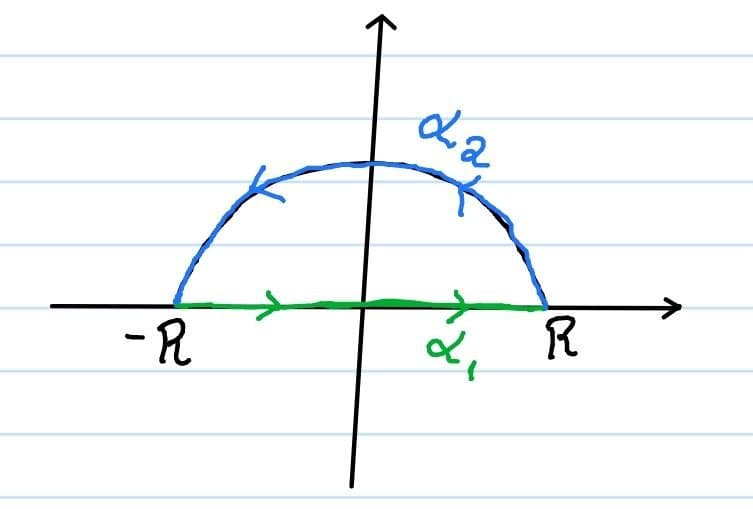
\includegraphics[scale=.4]{exemplo3.png}
    \caption{Curvas no semi-circulo}
    \label{fig:ex3}
\end{figure}

Como $z = x + yi,\ x, y \in \mathbb{R}$, em $\alpha_1$ temos $y = 0$. Assim tomando $R \to \infty$

\begin{equation*}
    \lim_{R \to \infty} \int_\alpha \frac{1}{z^4 + 4} d z = \lim_{R \to \infty} \int_{-R}^R \frac{1}{x^4 + 4} d x + \lim_{R \to \infty} \int_{\alpha_2} \frac{1}{z^4 + 4} d z
\end{equation*}

Temos 3 limites e um deles é o que queremos, então vamos calcular os outros 2

\begin{align*}
    \lim_{R \to \infty} \int_\alpha \frac{1}{z^4 + 4} d z &= \lim_{R \to \infty} \int_\alpha \frac{1}{(z - 1 -i)(z +1 - i)(z + 1 + i)(z - 1 + i)}d z \\
    &= \lim_{R \to \infty} \left( 2 \pi i \cdot \left( \mathrm{Res}_{z = 1 + i} f(z) + \mathrm{Res}_{z = - 1 + i} f(z) \right) \right) \\
    &= \lim_{R \to \infty} \left( 2 \pi i \cdot \left( \frac{- 1 - i}{16} + \frac{1 - i}{16} \right) \right) \\
    &= \lim_{R \to \infty} \left( \frac{\pi}{4} \right) = \frac{\pi}{4}
\end{align*}

E para o outro limite parametrizamos por $z(t) = R \cdot e^{i t}\ (0 \leq t \leq t)$

\begin{align*}
    \lim_{R \to \infty} \left| \int_{\alpha_2} \frac{1}{z^4 + 4}d z \right| &\leq \lim_{R \to \infty} \int_{\alpha_2} \frac{1}{R^4 + 4}d z \\
    &= \lim_{R \to \infty} \left( \frac{1}{R^4 + 4} \int_{\alpha_2} d z \right) \\
    &= \lim_{R \to \infty} \left( \frac{1}{R^4 + 4} \pi R \right) \\
    &= 0
\end{align*}

Ou seja,

$$\frac{\pi}{4} = I + 0$$

Logo, $I = \frac{\pi}{4}$
\end{ex}

\end{document}

